\documentclass[letterpaper,11pt]{article}
\oddsidemargin -1.0cm \textwidth 17.5cm

\usepackage[utf8]{inputenc}
\usepackage[activeacute,spanish]{babel}
\usepackage{amsfonts,setspace}
\usepackage{amsmath}
\usepackage{amssymb, amsmath, amsthm}
\usepackage{comment}
\usepackage{amssymb}
\usepackage{dsfont}
\usepackage{anysize}
\usepackage{multicol}
\usepackage{enumerate}
\usepackage{graphicx}
\usepackage[left=1.5cm,top=2cm,right=1.5cm, bottom=1.7cm]{geometry}
\setlength\headheight{1.5em} 
\usepackage{fancyhdr}
\usepackage{multicol}
\usepackage{hyperref}
\usepackage{wrapfig}
\pagestyle{fancy}
\fancyhf{}
\renewcommand{\labelenumi}{\normalsize\bfseries P\arabic{enumi}.}
\renewcommand{\labelenumii}{\normalsize\bfseries (\alph{enumii})}
\renewcommand{\labelenumiii}{\normalsize\bfseries \roman{enumiii})}

\begin{document}

\fancyhead[L]{\itshape{Facultad de Ciencias F\'isicas y Matem\'aticas}}
\fancyhead[R]{\itshape{Universidad de Chile}}

\begin{minipage}{11.5cm}
    \begin{flushleft}
        \hspace*{-0.6cm}\textbf{FI1000-6 Introducción a la Física Clásica}\\
        \hspace*{-0.6cm}\textbf{Profesora:} Paulina Lira\\
        \hspace*{-0.6cm}\textbf{Auxiliares:} Juan Cristóbal Castro \& Alejandro Silva\\
        \hspace*{-0.6cm}\textbf{Ayudantes:} Francisca Bórquez, Catalina Molina\\
    \end{flushleft}
\end{minipage}

\begin{picture}(2,3)
    \put(366,-4){
\includegraphics[scale=0.9]{2020-1/Imágenes/logo/dfi-fcfm.pdf}}
\end{picture}

\begin{center}
	\LARGE \bf Auxiliar \#9: Trabajo y Energía   \\
\end{center}

\vspace{-1cm}
\begin{enumerate}\setlength{\itemsep}{0.4cm}

\rfoot[]{pág. \thepage}

\item[]

\item Un bloque de masa M comienza a deslizar, desde una altura H, por un una cuña de ángulo característico $\alpha$. Si el coeficiente de roce es $\mu$, determine el trabajo de la fuerza de roce sobre el bloque. 
\begin{figure}[h!]
    \centering
    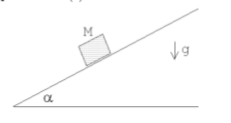
\includegraphics[scale=0.65]{2020-1/Imágenes/aux11/p1.png}
\end{figure}

\item En un parque de entretenciones un carro de masa m se desliza (sin roce) por una rampla desde un altura h (desconocida) ingresando a un loop de radio R. Para abaratar costos la altura h desde donde se suelta el carro es la mínima para que el carro no se suelte de la vía. Emergiendo del loop el carro entra a una zona de frenado de largo L (desconocido) que consiste en una plano con coeficiente de roce $\mu$. Sin embargo el carro no alcanza a frenar en la primera pasada, si no que pasa de largo y entra en contacto con un resorte de constante elástica k. Vuelve y reingresa a la zona de frenado donde se detiene justo en la mitad de este. Determine:
\begin{enumerate}
    \item Velocidad en el punto B
    \item Magnitud de h
    \item Largo L
    \item Máxima compresión del resorte
\end{enumerate}
\begin{figure}[h!]
    \centering
    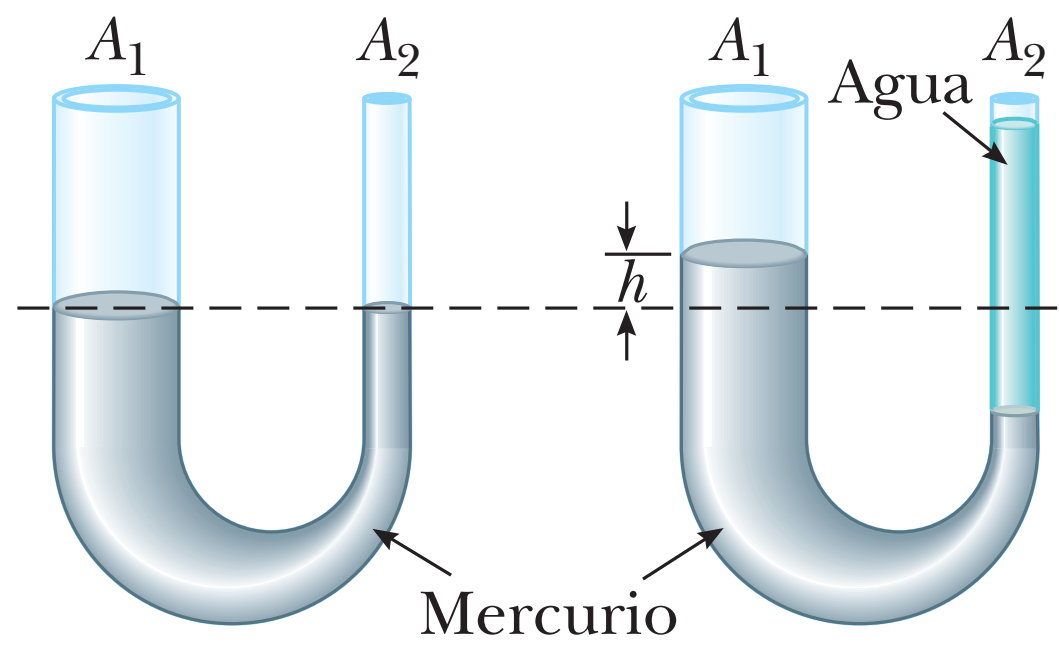
\includegraphics[scale=0.65]{2020-1/Imágenes/aux11/p2.png}
\end{figure}


\end{enumerate}
\end{document}